\documentclass{article}
%Preamble
\usepackage{float}
\usepackage{color}
\usepackage{listings}
\usepackage{longtable}
\usepackage{amsmath,amssymb}
\usepackage{graphics}
\usepackage{graphicx}

\title{AE 622 -  Computing of high speed flows\\ Assignment 3: Report \\ Capturing a normal shock using Steger- Warming flux splitting method}
\author{Vinod Kumar Metla - 130010048\\Aditi Taneja - 13D100026}
\date{\today}

\begin{document}
\pagenumbering{arabic}
\maketitle
\newpage
\section*{Introduction}
Formulation for flux calculation using the Steger-Warming flux splitting and Lax-Friedrich methods are derived followed by Normal shock simulated using Lax Friedrich method in octave and Steger Warming Flux-Splitting Method in fortran with initial conditions as - 
\newline
    $\begin{bmatrix}
    \rho_l \\ 
    u_l \\
    p_l \\
    T_l
    \end{bmatrix} = \begin{bmatrix}
    1.225 kg/m^3\\ 
    3401.74 m/s\\
    101.325 KPa\\
    288 K
    \end{bmatrix} $, 
\\
$\begin{bmatrix}
    \rho_r \\ 
    u_r \\
    p_r \\
    T_r
    \end{bmatrix} = \begin{bmatrix}
    7.0 kg/m^3\\ 
    595.3 m/s \\
    11804.362 KPa \\
    5871.6 K
    \end{bmatrix} $
\newline
Simulations are carried out by varying Grid size 200, 400, and 800. $\alpha$ in Lax Friedrich scheme is set to 0.5, and CFL number is set to 0.2. Their effects on $\rho$, u, p, T are shown in the graphs with corresponding relative error plots in u.

\section*{Dependencies}
\begin{enumerate}
\item Pdflatex 
\item Octave
\item Numpy
\item Matplotlib

\end{enumerate}
\newpage

\section*{Flux Formulation using Steger Warming Flux Splitting method and Lax Friedrich method}

\subsection*{Introduction}
\begin{figure}[H]   \label{figure}
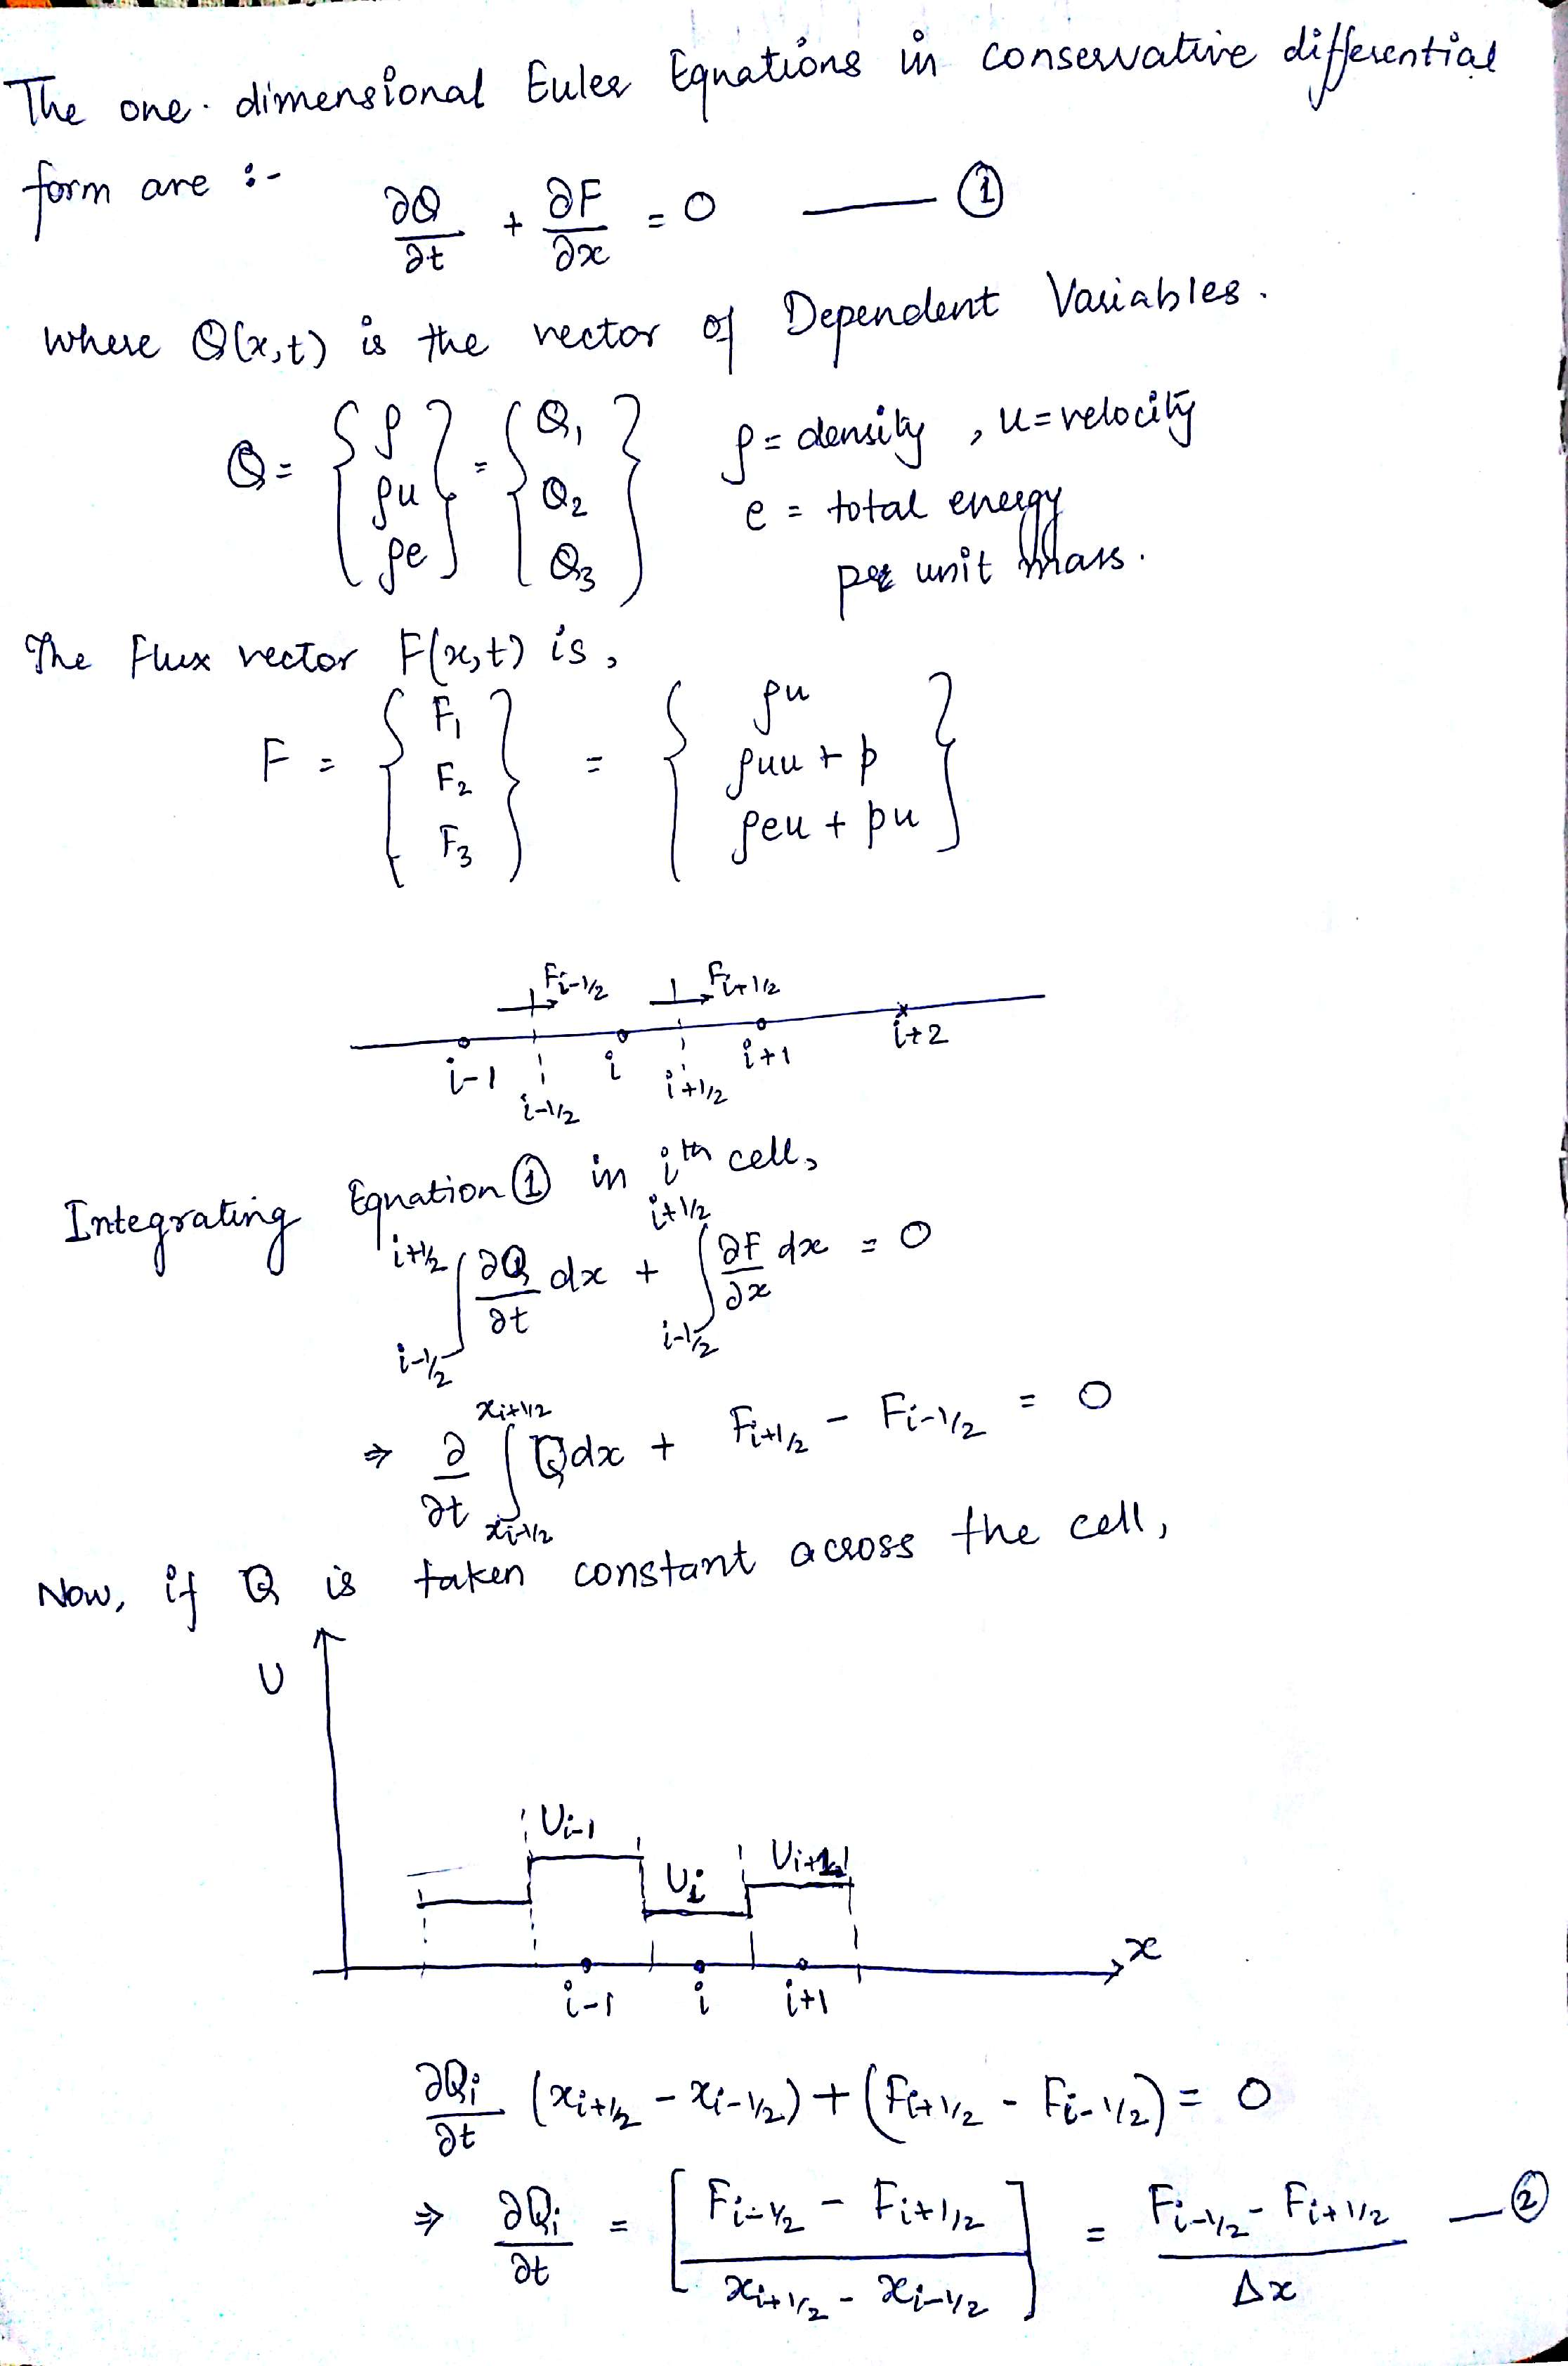
\includegraphics[width=14cm]{one.jpg}
\label{figure:}
\end{figure}
\newpage

\begin{figure}[H]   \label{figure}
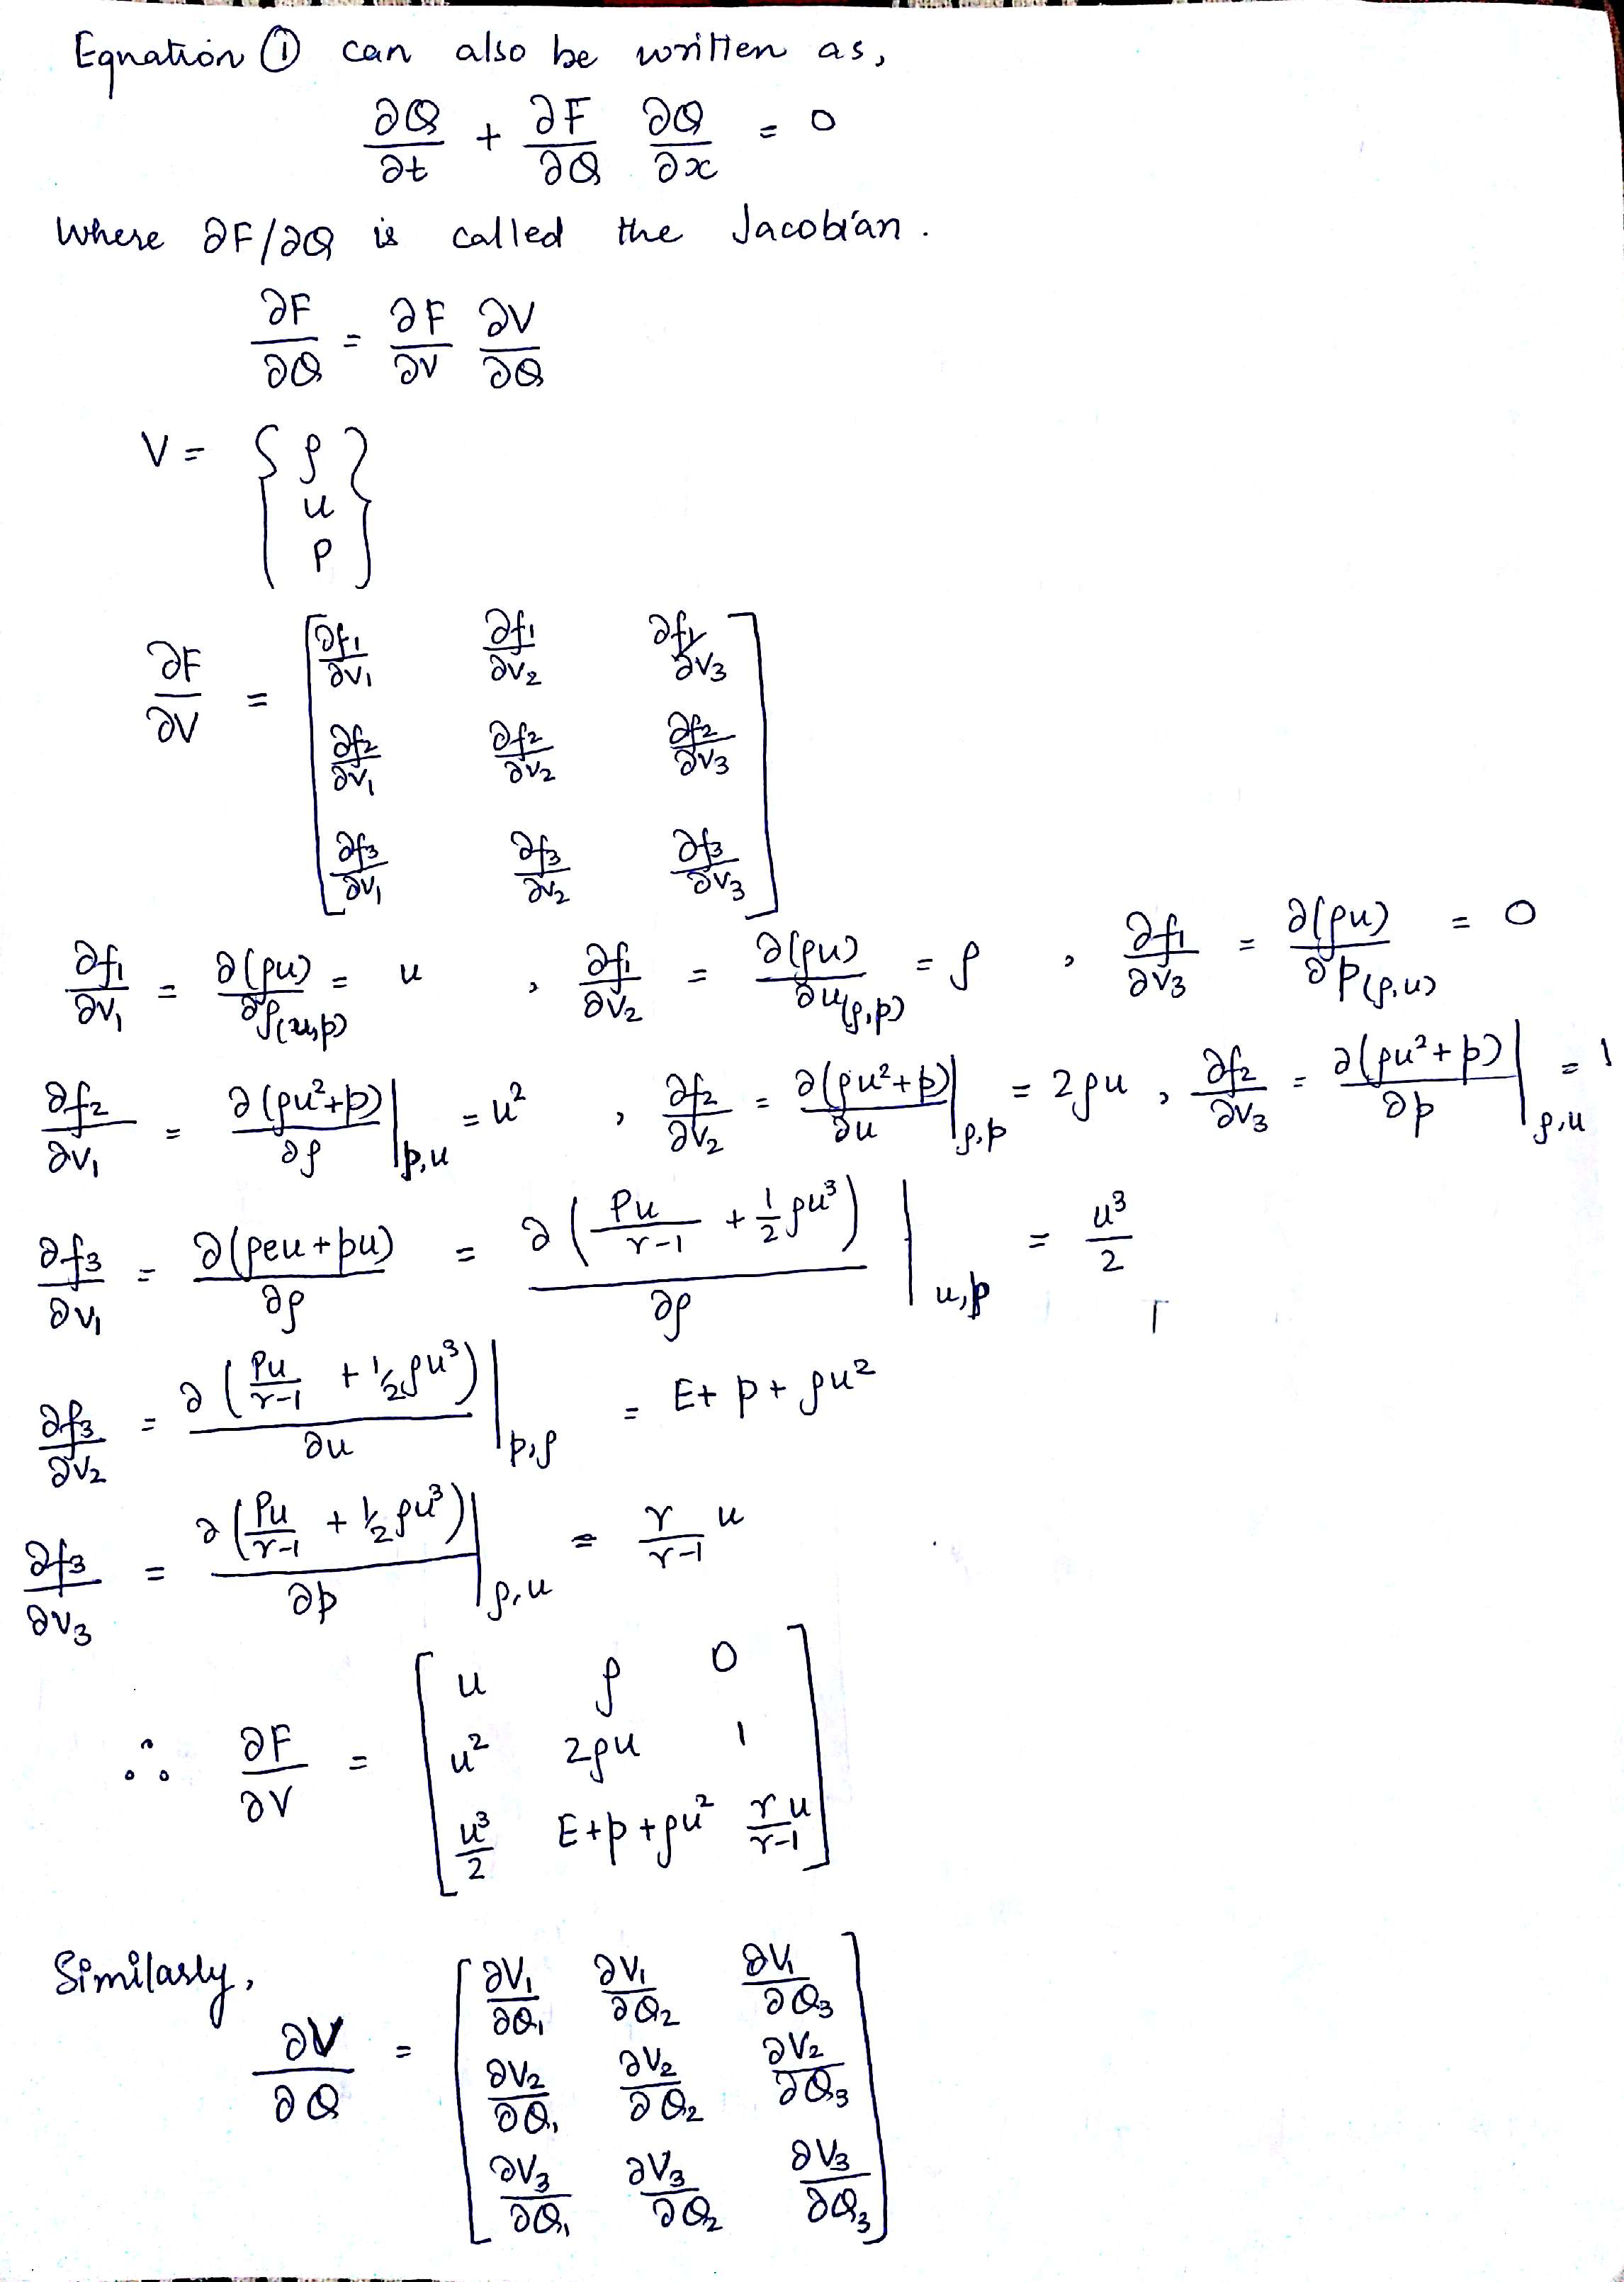
\includegraphics[width=15cm]{two.jpg}
\label{figure:}
\end{figure}
\newpage

\begin{figure}[H]   \label{figure}
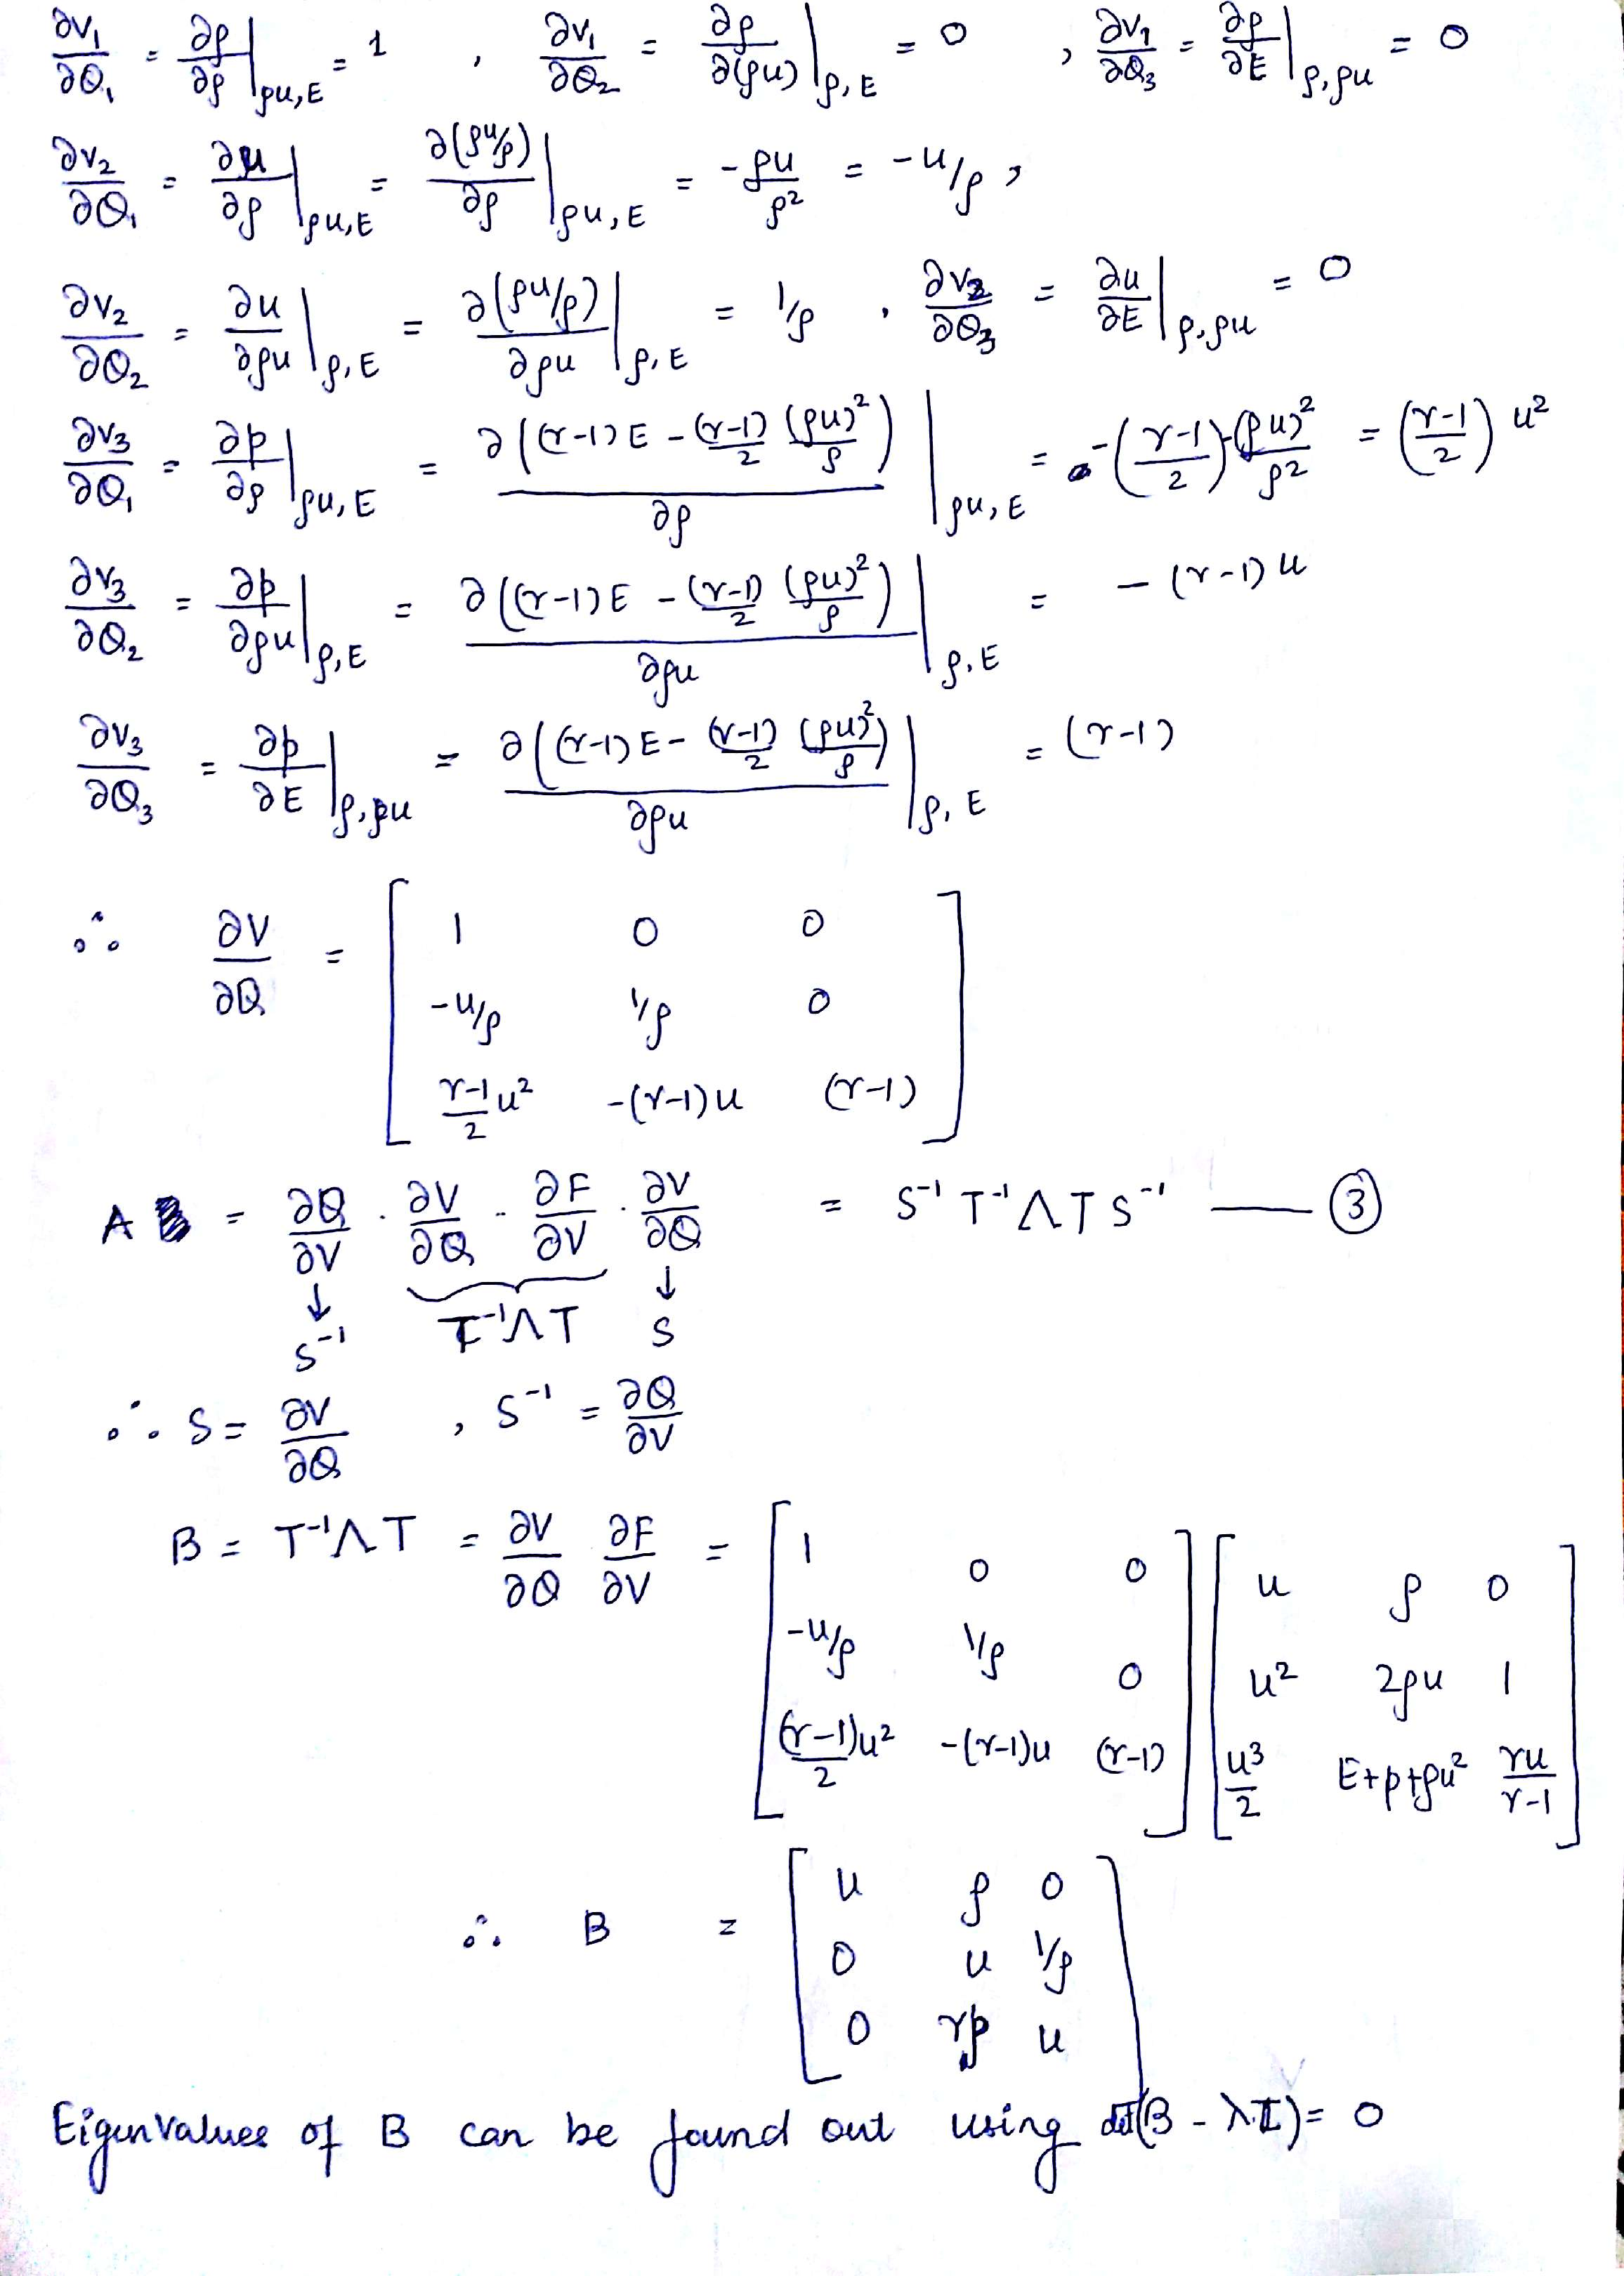
\includegraphics[width=15cm]{three.jpg}
\label{figure:}
\end{figure}
\newpage

\subsection*{Steger Warming Method}
\begin{figure}[H]   \label{figure}
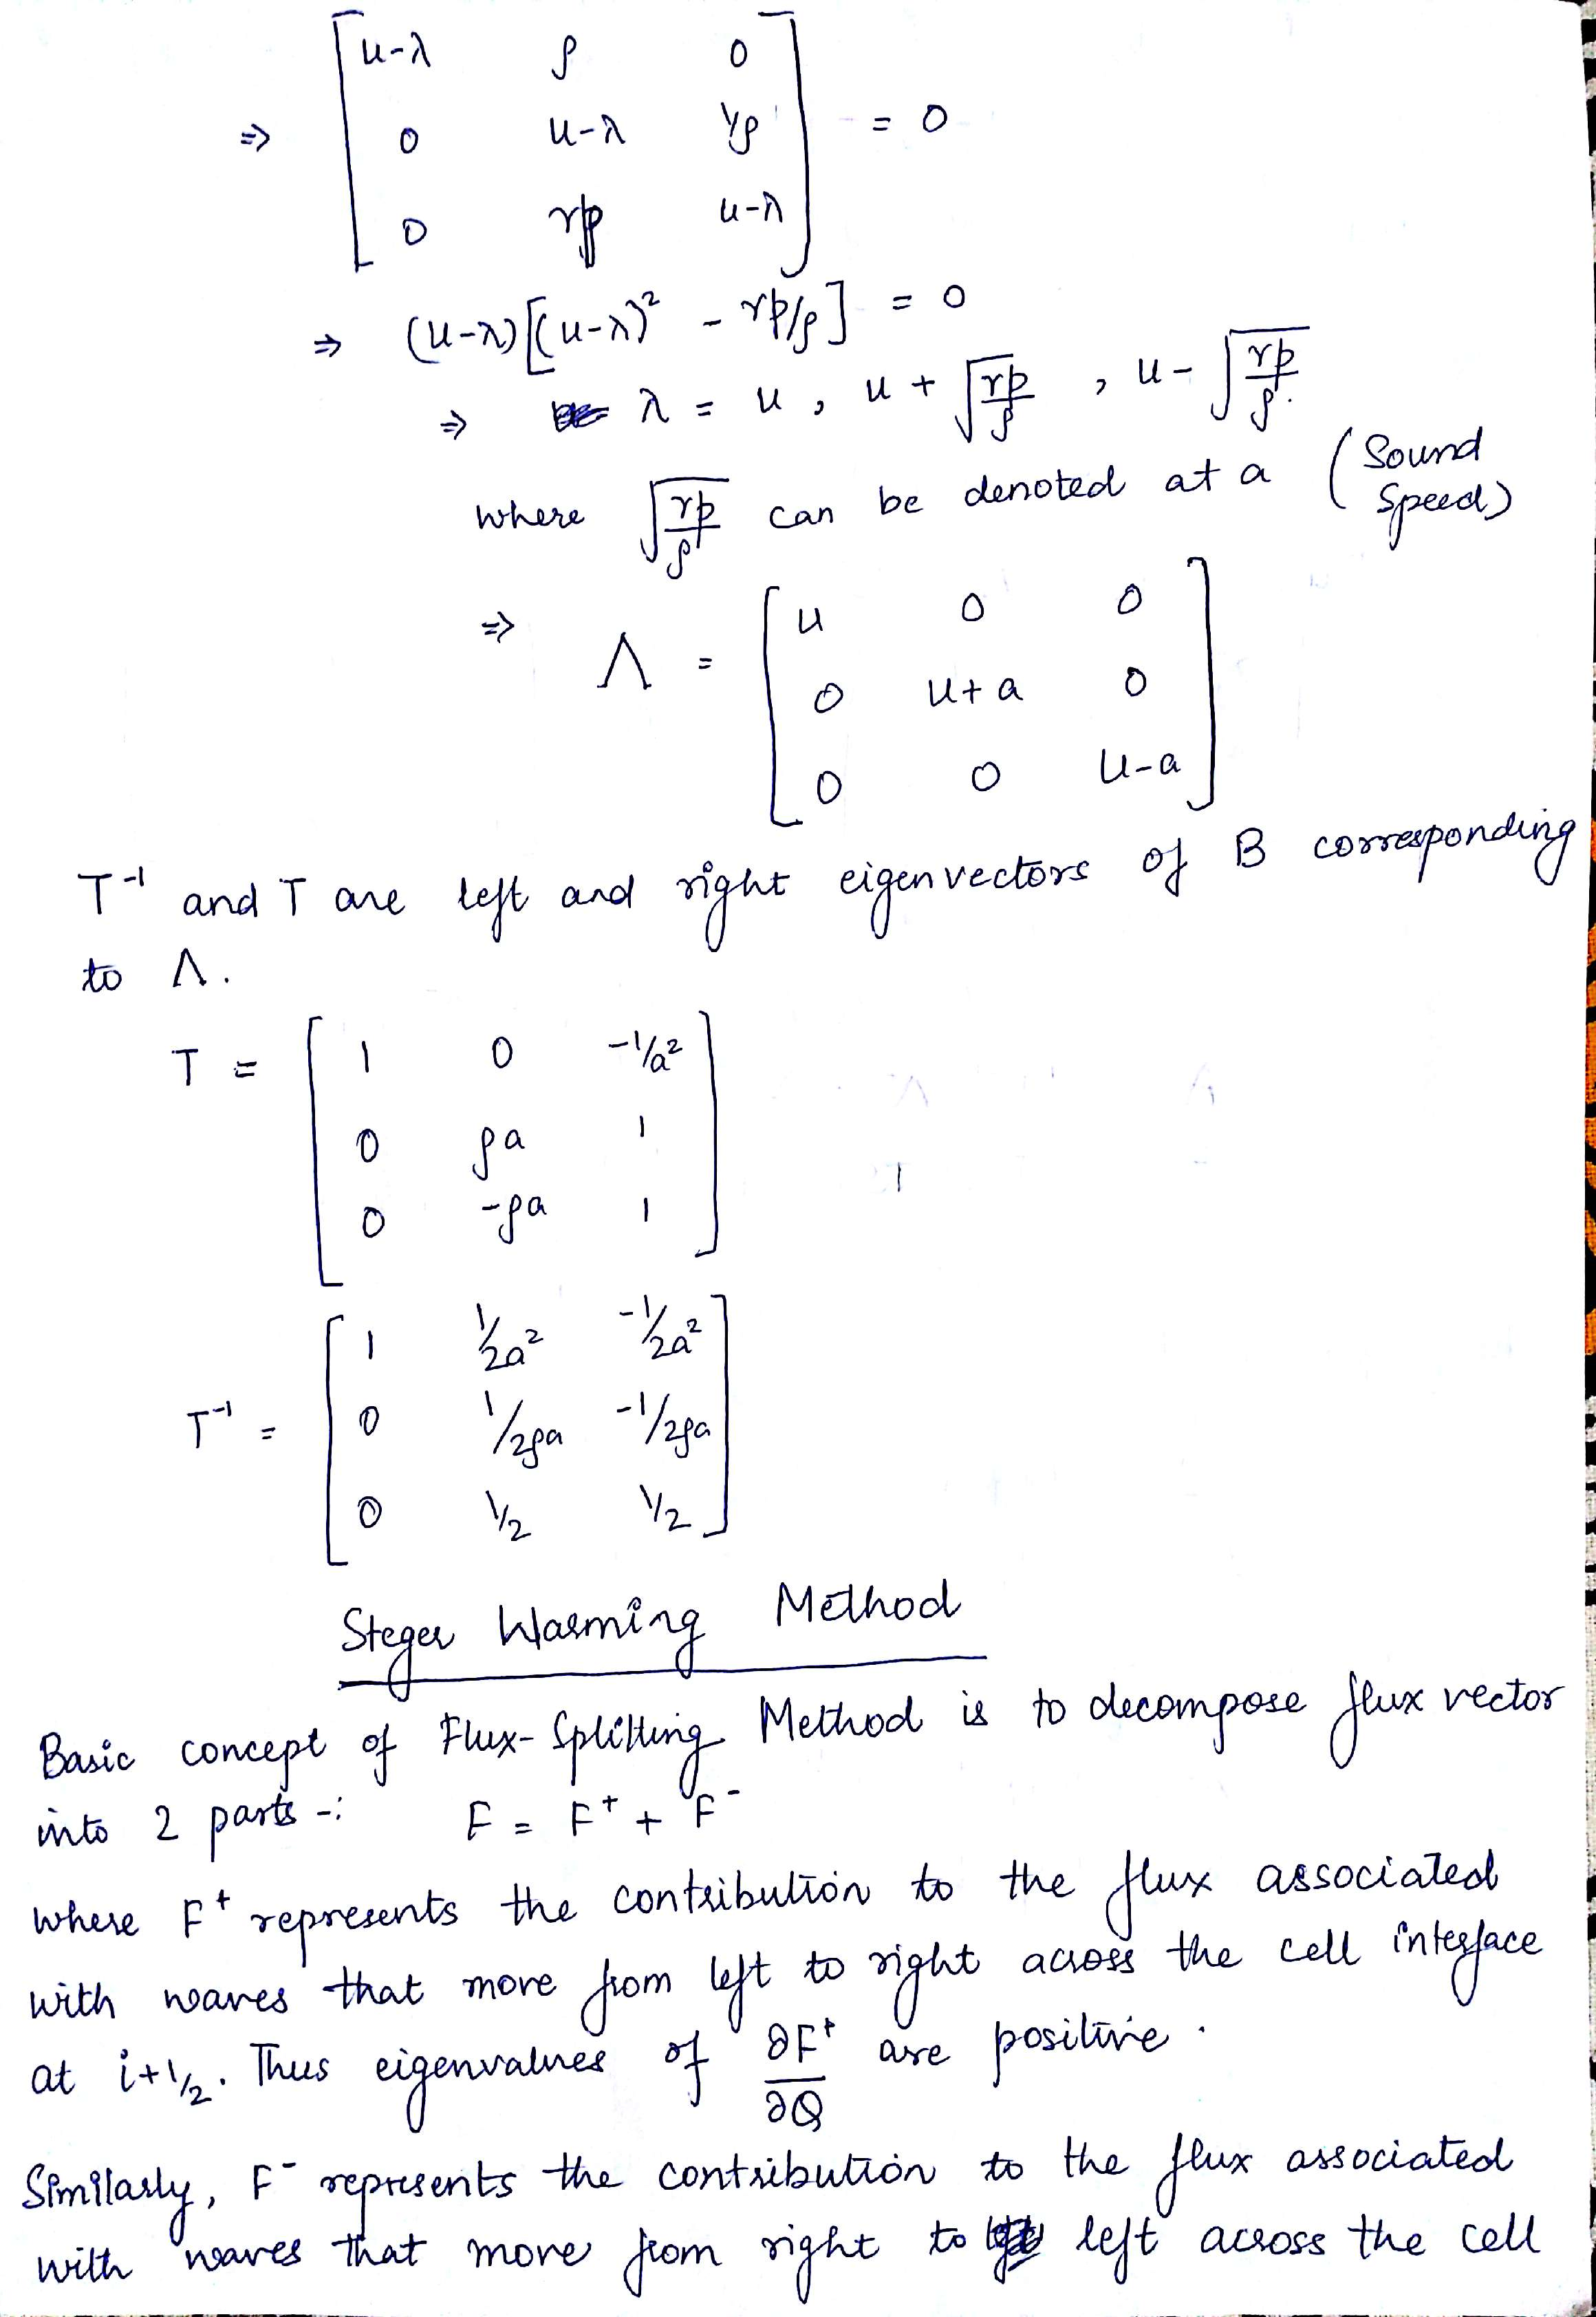
\includegraphics[width=15cm]{four.jpg}
\label{figure:}
\end{figure}
\newpage

\begin{figure}[H]   \label{figure}
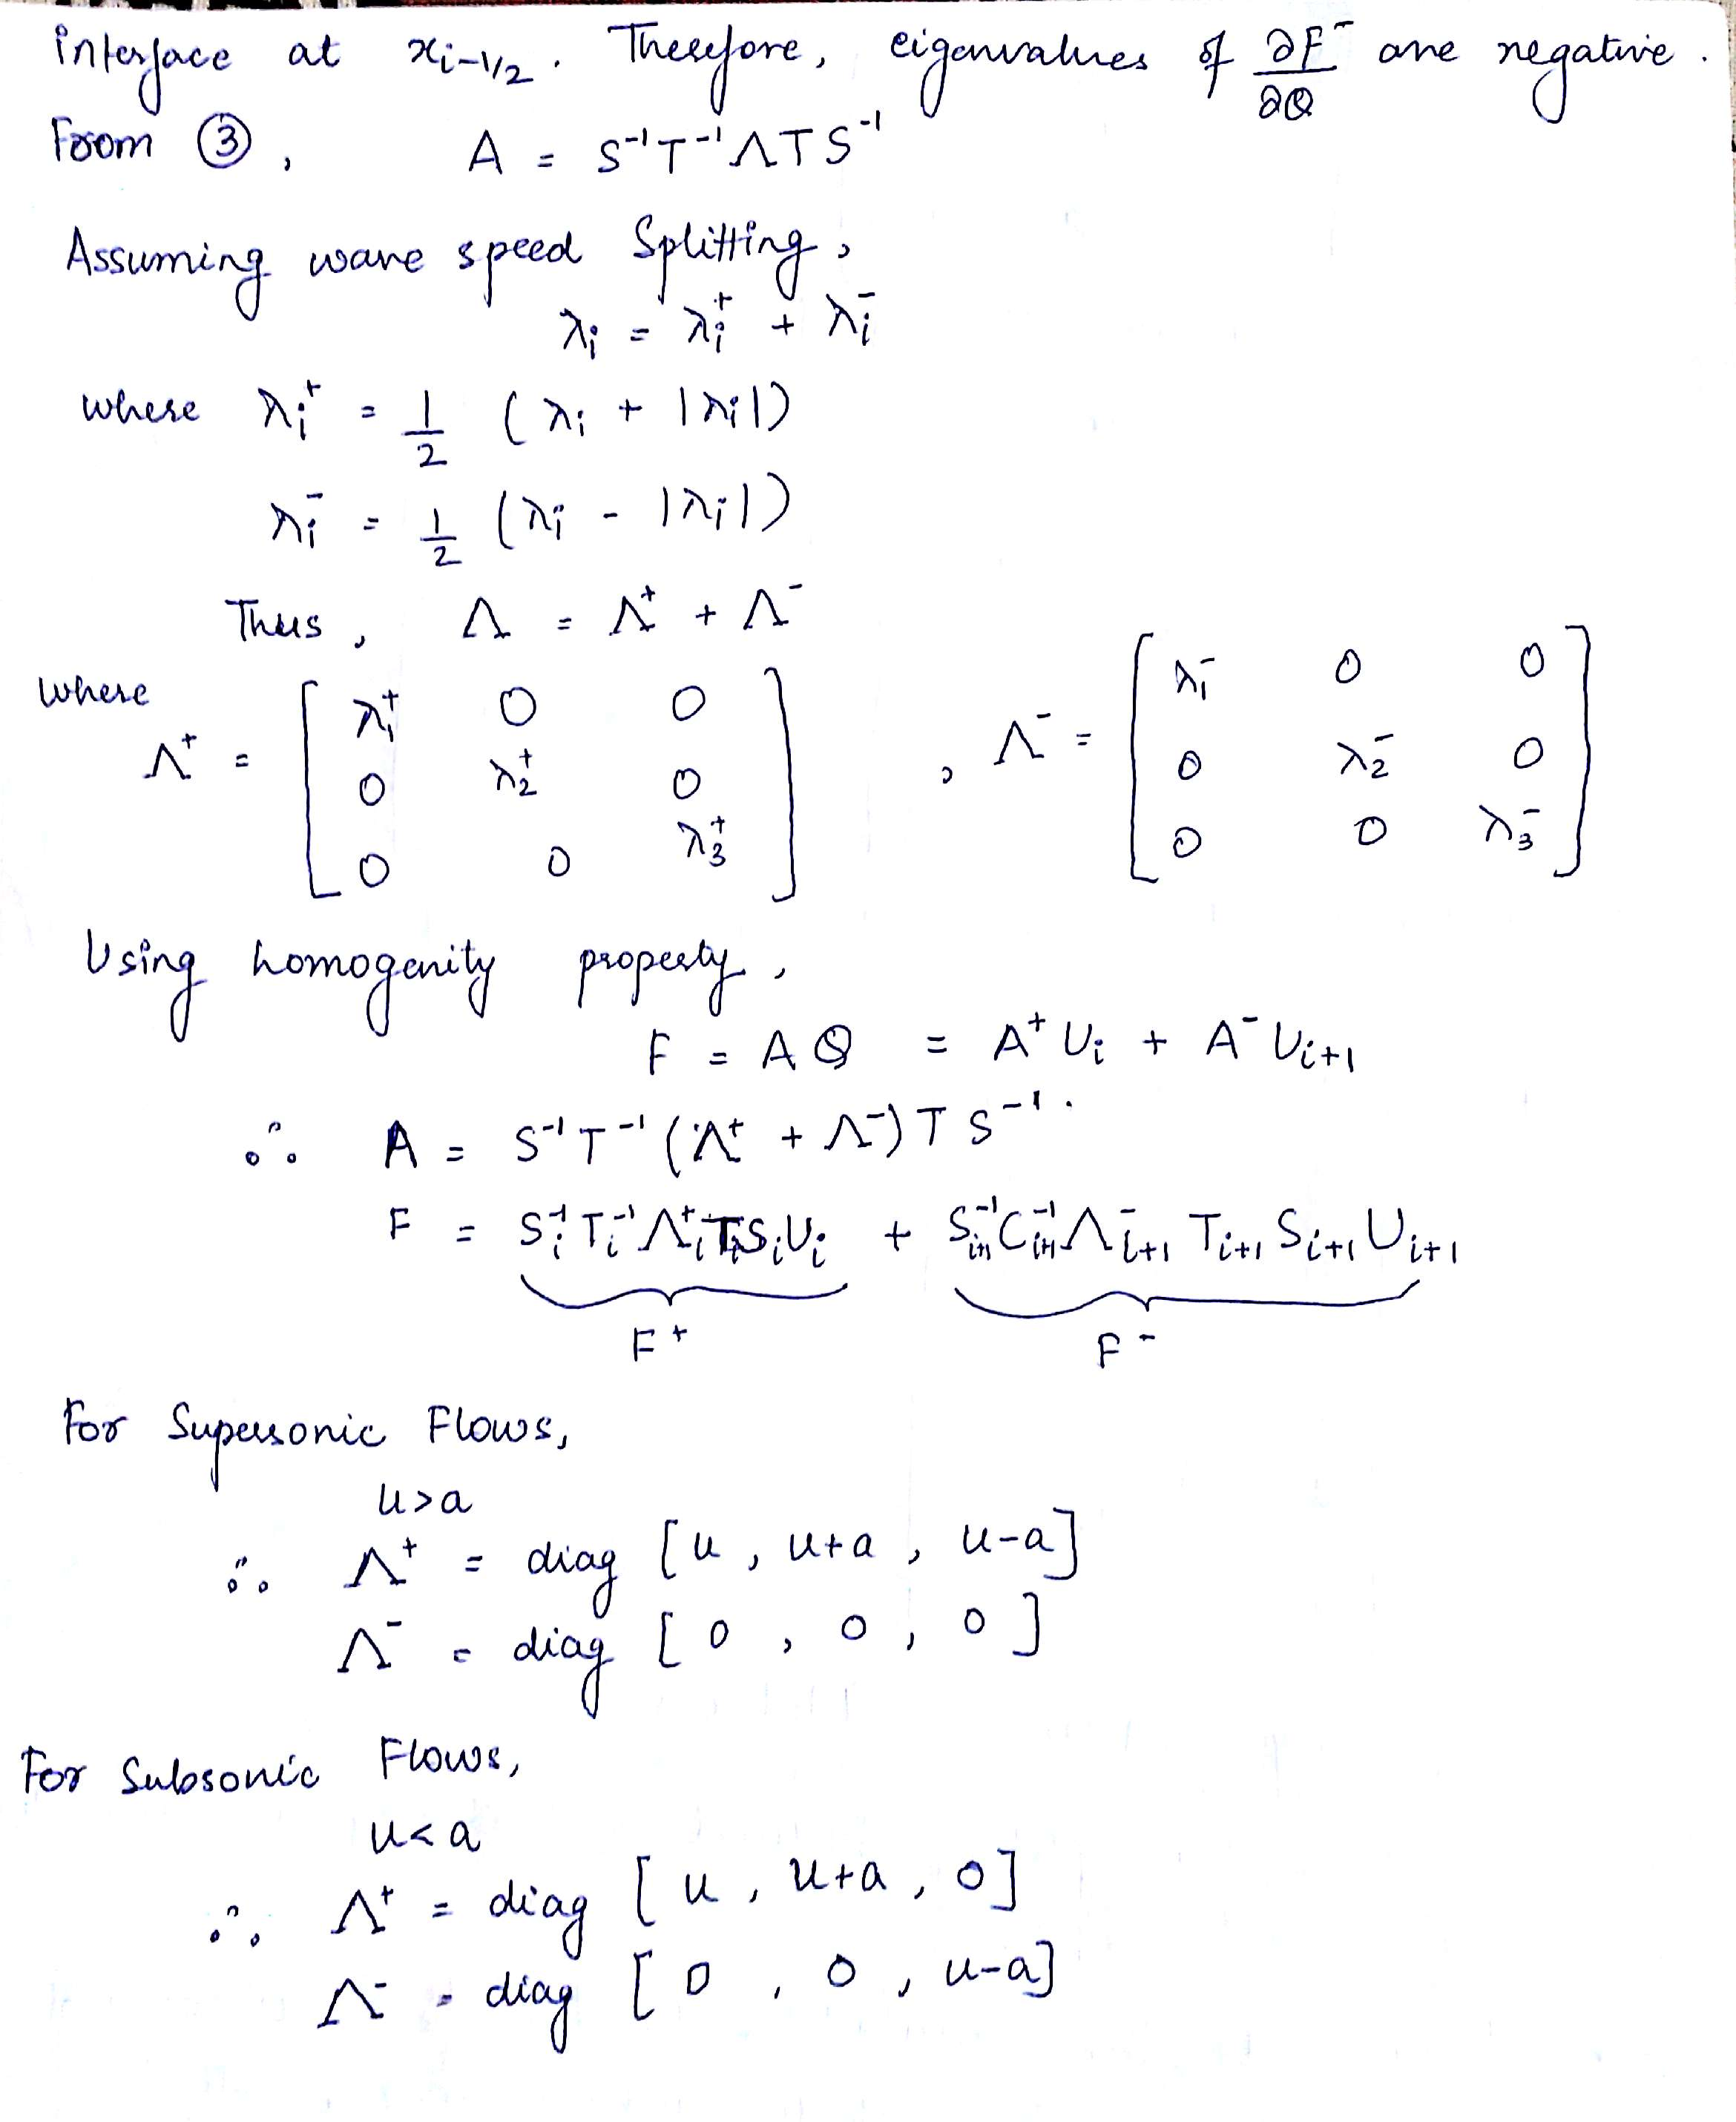
\includegraphics[width=15cm]{five.jpg}
\label{figure:}
\end{figure}
\newpage

\subsection*{Lax Friedrich Method}

\begin{figure}[H]   \label{figure}
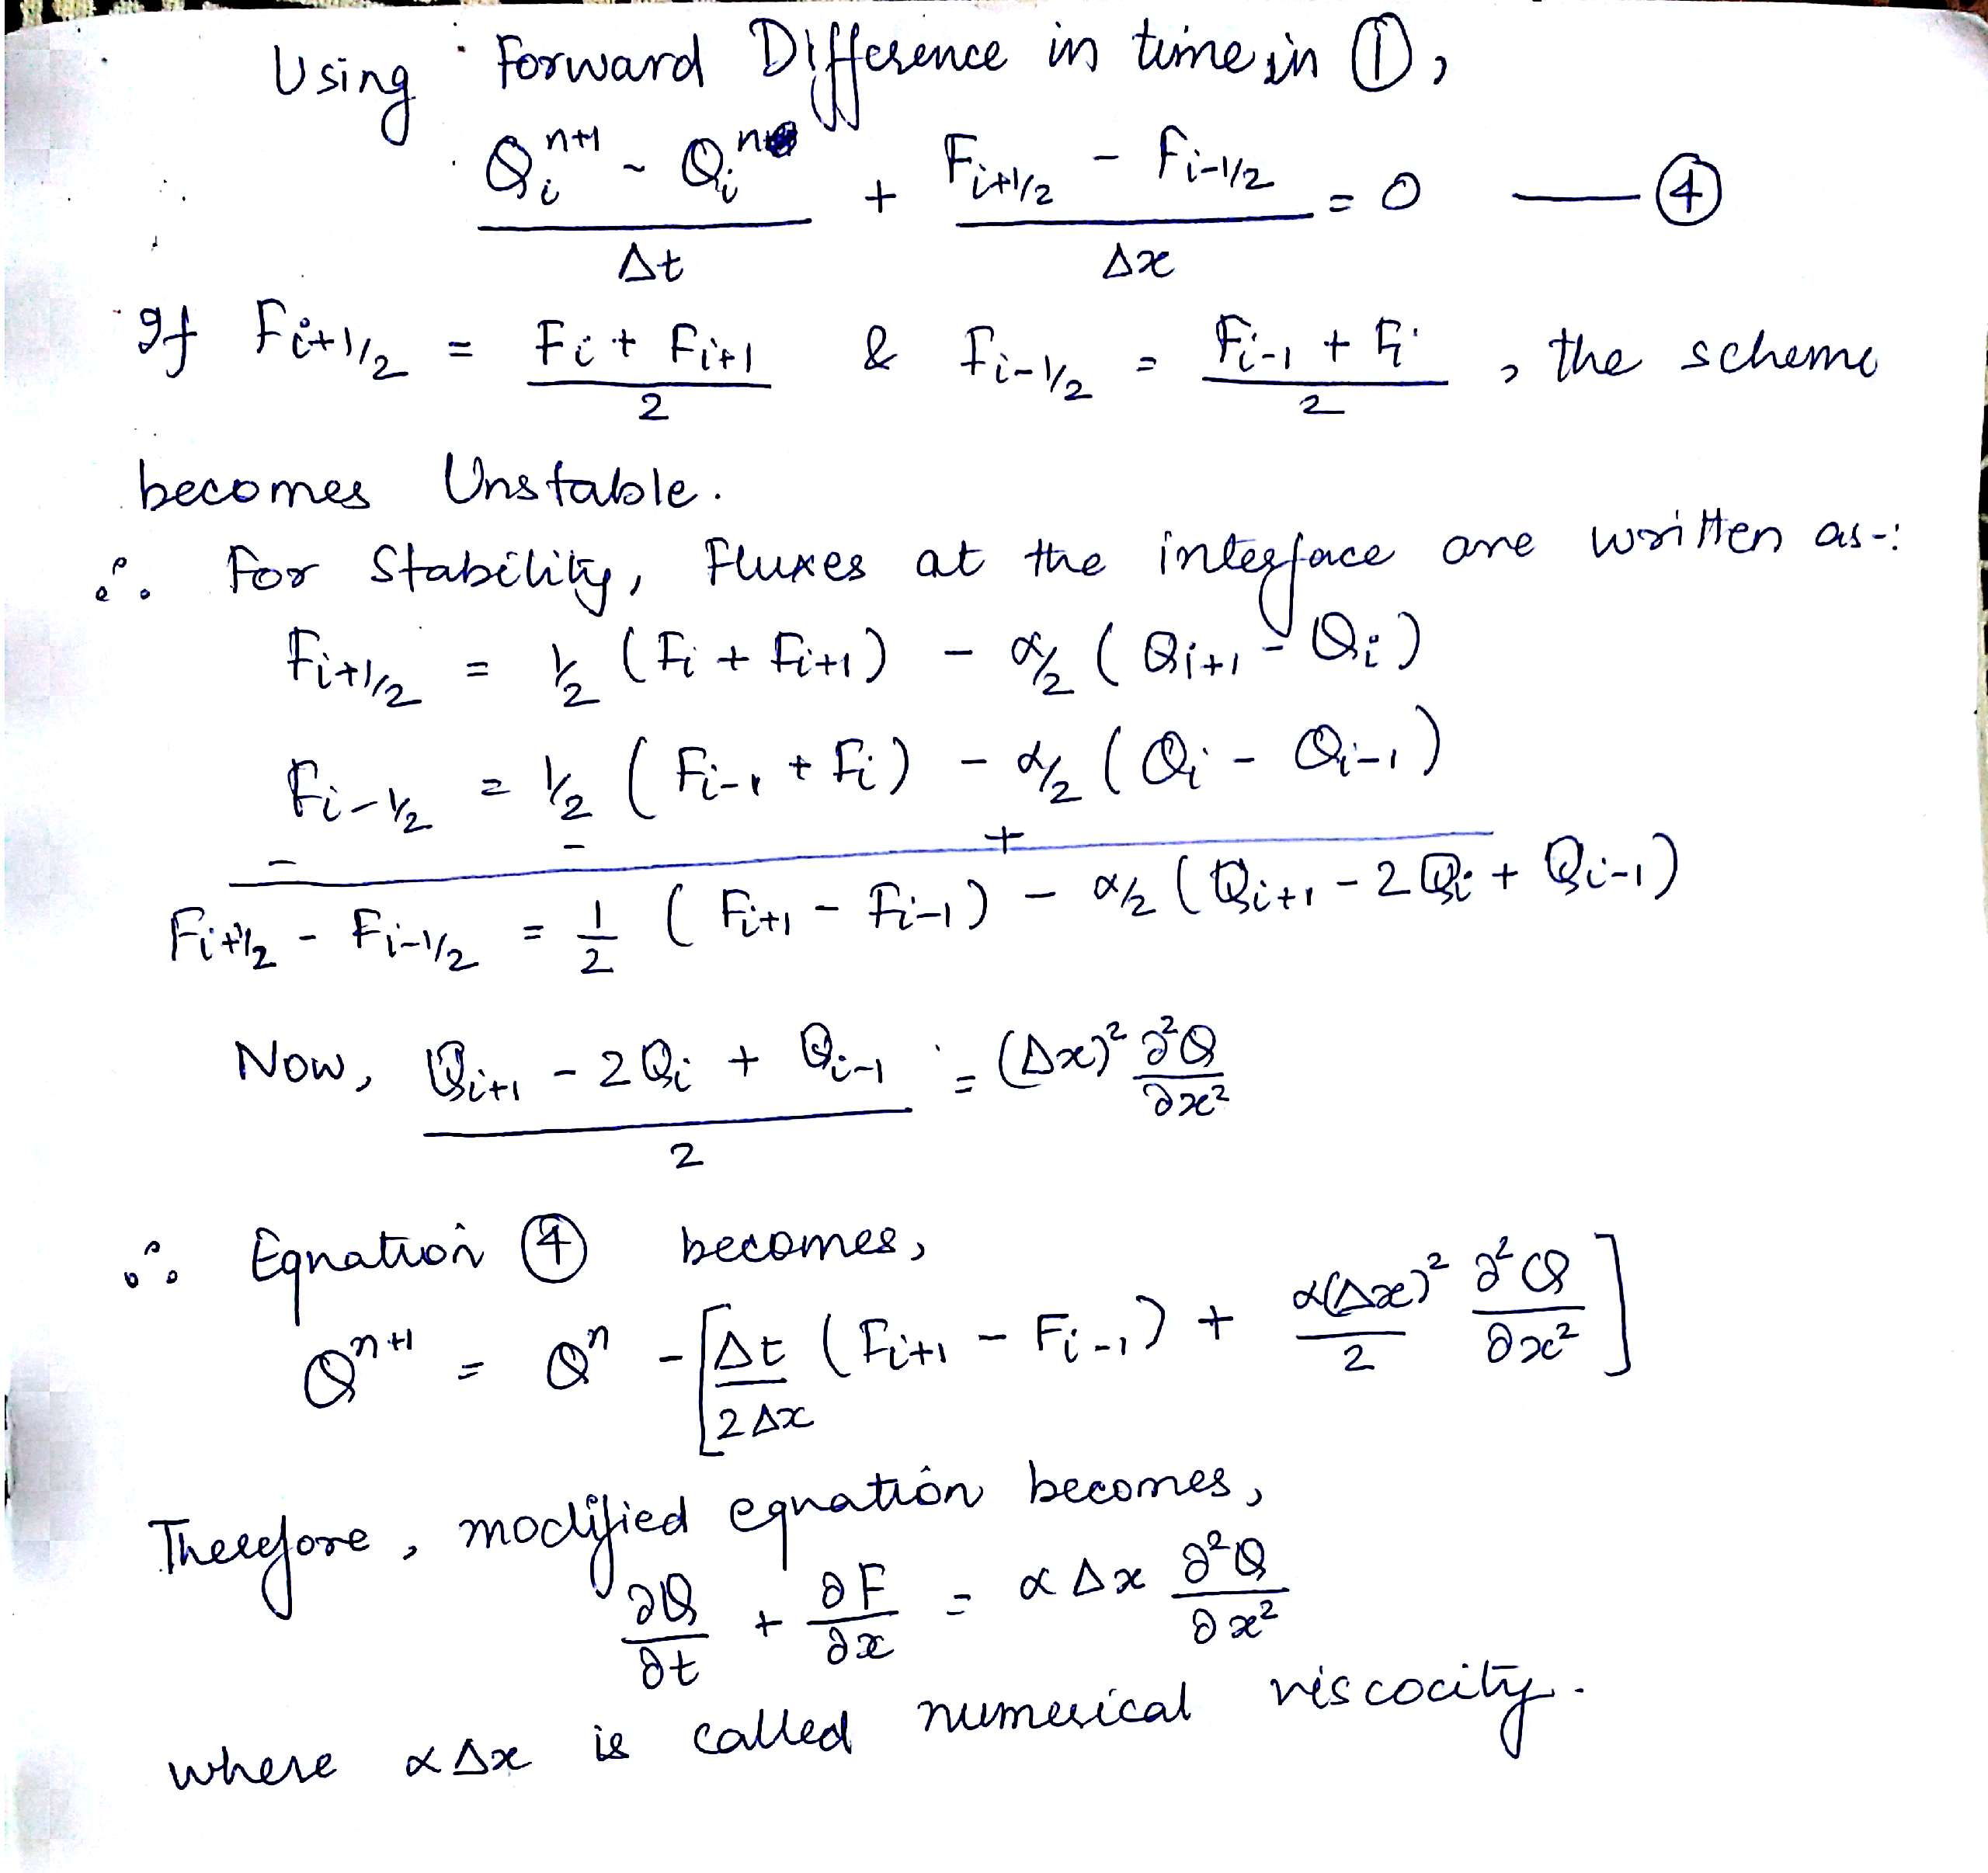
\includegraphics[width=15cm]{six.jpg}
\label{figure:}
\end{figure}
\newpage

\section*{Comparison Between Exact Solution and Approximate Methods}

\begin{figure}[H]   \label{figure}
\centering
\includegraphics[scale=0.6]{N_200.png}
\label{figure:}
\caption{Plot for comparison of exact solution and approximate solutions for normal shock with 200 Grid points}
\end{figure}
\newpage

\begin{figure}[H]   \label{figure}
\centering
\includegraphics[scale=0.6]{N_400.png}
\label{figure:}
\caption{Plot for comparison of exact solution and approximate solutions for normal shock with 400 Grid points}
\end{figure}
\newpage

\begin{figure}[H]   \label{figure}
\centering
\includegraphics[scale=0.6]{N_800.png}
\label{figure:}
\caption{Plot for comparison of exact solution and approximate solutions for normal shock with 800 Grid points}
\end{figure}
\newpage

\section*{Error Plots}

\begin{figure}[H]   \label{figure}
\centering
\includegraphics[scale=0.8]{Err_200.png}
\label{figure:}
\caption{Error in the solution using different schemes with 200 Grid points}
\end{figure}

\begin{figure}[H]   \label{figure}
\centering
\includegraphics[scale=0.8]{Err_400.png}
\label{figure:}
\caption{Error in the solution using different schemes with 400 Grid points}
\end{figure}

\begin{figure}[H]   \label{figure}
\centering
\includegraphics[scale=0.8]{Err_800.png}
\label{figure:}
\caption{Error in the solution using different schemes with 800 Grid points}
\end{figure}

\begin{figure}[H]   \label{figure}
\centering
\includegraphics[scale=0.5]{Err_per_length.png}
\label{figure:}
\caption{Error per unit length using different schemes with different grid points}
\end{figure}

\section*{Observations}

\begin{enumerate}
\item As the number of grid points increases solution converges to the exact solution in both Lax Friedrich method and Steger Warming method.

\item Few fluctuations are observed in the solution obtained by Lax Friedrich method, but there are negligible fluctuations observed in Steger Warming method. Therefore, there is less dispersion effects in Steger Warming than Lax Friedrich method.

\item In Error plots, band is decreasing in both methods. There is only a small change observed in magnitude of error in Steger Warming method, whereas in Lax Friedrich method, the magnitude decreases as the number of grid points increase. So, for lower number of grid points Steger Warming method gives a better approximate solution compared to the Lax Friedrich method, hence reducing computation cost.

\item In Steger warming method, most of the error is present after the shock and concentrated in a very small region whereas in Lax Friedrich method, the error is diffused across the shock. Due to this reason, there is a drastic increase in the error in Steger Warming method just after the shock. 
\item Error per unit length remains almost same in Steger warming method even though the number of grid points is increased, whereas for Lax Friedrich method, error decreases as number of grid points increase. Diffusion effect also decreases as number of grid points are increased in LF method.

\end{enumerate}


\end{document}
